\documentclass[11pt,a4paper,twoside]{report}

\usepackage[a4paper,inner=3cm,outer=2.5cm,top=2.7cm,bottom=2.7cm]{geometry}
\usepackage{microtype}
\usepackage{graphicx}
\usepackage{booktabs}
\usepackage{array}
\usepackage{tabularx}
\usepackage{float}
\usepackage{enumitem}
\usepackage{xcolor}
\usepackage{amsmath}
\usepackage{listings}
\usepackage{fancyhdr}
\usepackage{titlesec}
\usepackage{caption}
\usepackage{subcaption}
\usepackage[hidelinks]{hyperref}
\usepackage{tikz}
\usetikzlibrary{shapes.geometric,arrows.meta,positioning,fit,calc}

\definecolor{brand}{HTML}{4F46E5}
\definecolor{codebg}{HTML}{F4F5F9}


\lstset{basicstyle=\ttfamily\footnotesize,backgroundcolor=\color{codebg},frame=single,
  rulecolor=\color{black!15},breaklines=true,showstringspaces=false,keywordstyle=\color{brand}\bfseries,
  language=Python,columns=fullflexible,xleftmargin=2pt,xrightmargin=2pt}

\titleformat{\chapter}[display]{\normalfont\huge\bfseries}{\chaptertitlename\ \thechapter}{14pt}{\Huge}
\titlespacing*{\chapter}{0pt}{-10pt}{26pt}

\newcommand{\course}{UCS503 -- Software Engineering}
\pagestyle{fancy}
\fancyhf{}
\fancyhead[LE]{\thepage\quad \course}
\fancyhead[RO]{\course\quad \thepage}
\renewcommand{\headrulewidth}{0.4pt}
\fancypagestyle{plain}{\fancyhf{}\fancyfoot[C]{\thepage}\renewcommand{\headrulewidth}{0pt}}

\tikzset{
  box/.style={rectangle,draw=black!60,rounded corners=3pt,minimum height=0.9cm,minimum width=2.6cm,align=center,font=\small,fill=blue!7},
  ml/.style={rectangle,draw=black!60,rounded corners=3pt,minimum height=0.9cm,minimum width=2.6cm,align=center,font=\small,fill=violet!10},
  db/.style={cylinder,shape border rotate=90,aspect=0.25,draw=black!60,minimum height=1.1cm,minimum width=1.9cm,align=center,font=\small,fill=green!10},
  arr/.style={-{Latex[length=2.2mm]},thick,black!70}
}

\begin{document}

%% ------------------------------------------------------------------ title page
\begin{titlepage}
\centering
{\large \course\par}
\vspace{2.2cm}
{\Huge\bfseries CodeShield\par}
\vspace{0.4cm}
{\Large Hybrid AST and Machine-Learning Vulnerability Detection\\ and Risk Assessment Platform for Python\par}
\vspace{2.2cm}
{\large\bfseries Submitted by:\par}
\vspace{0.3cm}
\begin{tabular}{ll}
1024030152 & Rhea Balamurugan\\
1024030161 & Ishi Govil\\
1024030718 & Shreya Kush
\end{tabular}\\[0.6cm]
Group: \textbf{3C16} \quad BE Third Year, COE\par
\vspace{1.4cm}
{\large\bfseries Submitted to:\par}
\vspace{0.2cm}
Ms.\ Paramveer Kaur\par
\vfill
{\large\bfseries Mid-Semester Evaluation\par}
\vspace{0.4cm}
Computer Science and Engineering Department\\
Thapar Institute of Engineering and Technology, Patiala\par
\vspace{0.3cm}
2026
\end{titlepage}

\clearpage
\pagenumbering{roman}
\tableofcontents
\clearpage
\listoffigures
\clearpage
\listoftables
\clearpage
\pagenumbering{arabic}

%% ================================================================== CHAPTER 1
\chapter{Introduction}

\section{Background and Context}
Security flaws in source code are among the most expensive defects in software: they usually produce no visible runtime error, stay dormant until an attacker finds them, and are far cheaper to fix during development than after deployment. Injection flaws, broken authentication, cryptographic failures and security misconfiguration continue to appear in the OWASP Top~10 \cite{owasp2021}, and each can be mapped to a Common Weakness Enumeration (CWE) entry \cite{cwe}.

Two families of automated tools address this problem. \emph{Rule-based static analysers} such as Bandit \cite{bandit} and Semgrep \cite{semgrep} are fast and explainable but only detect the patterns someone wrote a rule for. \emph{Machine-learning detectors} \cite{russell2018,fan2020} generalise across code variants, but are typically opaque, need large datasets, and give no precise location. CodeShield combines both: an AST-based static engine with data-flow (taint) tracking, and a calibrated, explainable machine-learning classifier whose output is fused into one scored, actionable report shown in a web dashboard.

This report covers the work done up to the mid-semester evaluation. Compared with the earlier prototype (five vulnerability classes, regular-expression rules, a 399-sample dataset and a mock-data fallback in the user interface) the system has been redesigned end-to-end: a new analysis engine, an extended multi-source dataset and model, a persistent REST API, and a completely rebuilt front end.

\subsection{Problem Statement}
Developers need a tool that (i) finds a broad range of security weaknesses in Python code without drowning them in false alarms, (ii) points to the exact line and explains why the code is dangerous, (iii) suggests a secure fix, and (iv) prioritises findings so critical issues are fixed first. Existing pattern-matching tools miss variants (for example an f-string SQL query built on a previous line) while pure ML tools cannot say \emph{where} the problem is. The project's central question is whether combining static analysis with an ML model gives better detection than either alone, \emph{measured honestly} on code that was not used for training.

\section{Project Objectives}
\begin{enumerate}[noitemsep]
  \item \textbf{Broaden coverage:} detect 12 vulnerability classes (up from 5) mapped to CWE and OWASP categories.
  \item \textbf{Accurate static analysis:} replace line-by-line regular expressions with AST analysis and taint tracking; remove false positives on comments and safe, parameterised code.
  \item \textbf{Handle diverse code:} build a larger, multi-source dataset (target $>$2{,}000 samples) and train a model that generalises to unseen sources.
  \item \textbf{Hybrid decision:} fuse static and ML outputs into a single severity, confidence and risk score, with an explanation for every finding.
  \item \textbf{Presentable product:} a persistent REST API and a polished React dashboard with scan history, statistics, report export and a model-transparency page.
  \item \textbf{Evaluate honestly:} use group-aware splits, cross-source tests and a static/ML/hybrid ablation; document limitations.
\end{enumerate}
These objectives are specific, measurable (class count, dataset size, F1/recall/false-positive rate) and were achieved within the semester timeline (Section~\ref{sec:analysis}).

\section{Scope and Limitations}
CodeShield analyses \textbf{Python} source code at file, function and snippet level. It is a decision-support tool: it does not execute scanned code, does not perform whole-program inter-procedural analysis, and cannot guarantee the absence of vulnerabilities. Findings must be reviewed by a developer.

%% ================================================================== CHAPTER 2
\chapter{Methodology and Design}

\section{System Architecture}

\subsection{High-Level Design}
CodeShield follows a three-tier architecture (Figure~\ref{fig:arch}). The \emph{presentation tier} is a single-page React application. The \emph{service tier} is a FastAPI application exposing a REST API; its core is the scan pipeline, which runs the static analyser and the ML engine and fuses their outputs. The \emph{data tier} is an SQLite database that stores every scan so that it can be re-opened, exported and aggregated on the dashboard.

\begin{figure}[H]
\centering
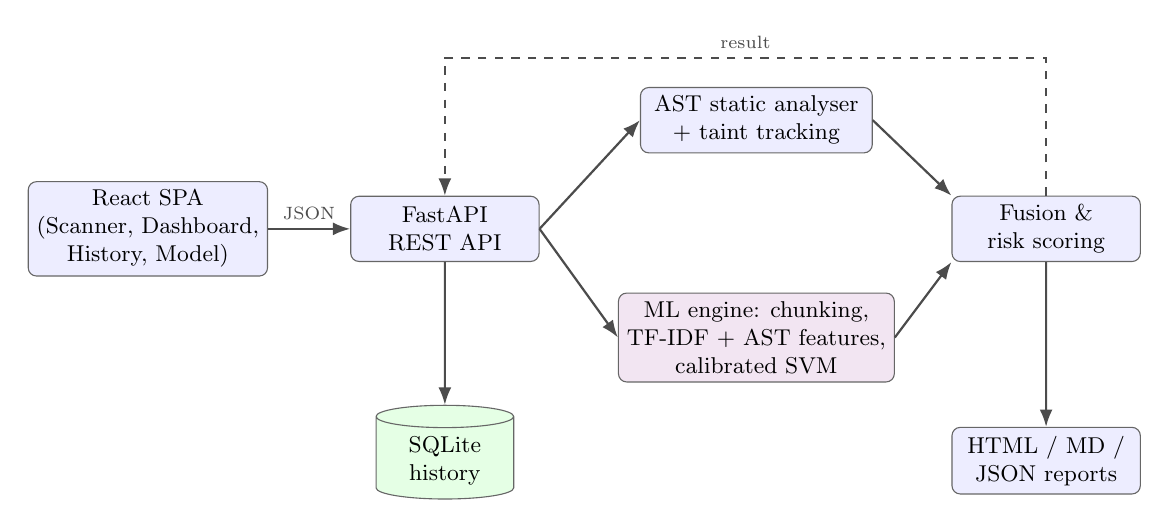
\begin{tikzpicture}[scale=0.92,transform shape]
  \node[box] (ui) at (0,0) {React SPA\\(Scanner, Dashboard,\\History, Model)};
  \node[box] (api) at (4.1,0) {FastAPI\\REST API};
  \node[box,minimum width=3.2cm] (st) at (8.4,1.5) {AST static analyser\\+ taint tracking};
  \node[ml,minimum width=3.2cm] (mlx) at (8.4,-1.5) {ML engine: chunking,\\TF-IDF + AST features,\\calibrated SVM};
  \node[box] (fus) at (12.4,0) {Fusion \&\\risk scoring};
  \node[db] (db) at (4.1,-3.2) {SQLite\\history};
  \node[box] (rep) at (12.4,-3.2) {HTML / MD /\\JSON reports};
  \draw[arr] (ui) -- node[above,font=\scriptsize]{JSON} (api);
  \draw[arr] (api.east) -- (st.west); \draw[arr] (api.east) -- (mlx.west);
  \draw[arr] (st.east) -- (fus.north west); \draw[arr] (mlx.east) -- (fus.south west);
  \draw[arr] (api) -- (db); \draw[arr] (fus) -- (rep);
  \draw[arr,dashed] (fus.north) -- ++(0,1.9) -| node[above,pos=0.25,font=\scriptsize]{result} (api.north);
\end{tikzpicture}
\caption{CodeShield architecture: request flow from the browser through the hybrid analysis pipeline.}
\label{fig:arch}
\end{figure}

\paragraph{Scan flow.} (1) The browser posts the source to \texttt{POST /api/scan}. (2) The code is normalised and parsed into an AST; if parsing fails a lexical fallback is used. (3) The static analyser walks the tree, tracks tainted values and emits findings with line, CWE, confidence and a data-flow trace. (4) In parallel the ML engine splits the file into functions or statement groups, vectorises each block and predicts class probabilities. (5) The fusion step boosts findings both engines agree on, adds ML-only findings above a probability threshold, localises them using evidence tokens, and computes severity and a 0--100 risk score. (6) The result is stored in SQLite and returned to the UI.

\subsection{Technical Stack}
\begin{itemize}[noitemsep]
  \item \textbf{Languages/frameworks:} Python~3.12, FastAPI \cite{fastapi} + Pydantic v2 (API), TypeScript + React~18 + Vite (UI), Tailwind CSS.
  \item \textbf{Database:} SQLite (standard library) for scan history and statistics.
  \item \textbf{ML:} scikit-learn~1.9 \cite{sklearn} (TF-IDF, LinearSVC, probability calibration, grouped cross-validation), NumPy, pandas.
  \item \textbf{UI libraries:} CodeMirror~6 (editor with line markers), Recharts (charts), React Router, Lucide icons.
  \item \textbf{Tools:} pytest + FastAPI TestClient (43 tests), Bandit and Semgrep rule suites (data), Docker (backend image), Git.
\end{itemize}

\section{Implementation Details}

\subsection{Module 1: Extended Dataset}
The first prototype used 399 samples (OWASP Benchmark for Python \cite{owaspbench} and a vulnerability-remediation set). Auditing it revealed two problems: more than half of the rows began with an identical OWASP licence header, and many rows were near-duplicates of one another, so a random split leaks information and inflates accuracy. The new dataset (Table~\ref{tab:data}) combines four public sources:
\begin{itemize}[noitemsep]
  \item \textbf{CodeShield v1} -- 398 usable samples (OWASP Benchmark for Python, Python Vulnerability Remediation).
  \item \textbf{SecurityEval} \cite{siddiq2022} -- 68 insecure samples with CWE ids.
  \item \textbf{Semgrep rule test-suites} \cite{semgrep} -- 1{,}081 samples extracted from \texttt{\# ruleid:} (vulnerable) and \texttt{\# ok:} (safe, hard-negative) annotations; the rule's CWE metadata gives the class.
  \item \textbf{Bandit examples} \cite{bandit} -- 371 samples labelled by running Bandit and mapping its test ids to classes.
  \item \textbf{Benign background corpus} -- 520 ordinary functions sampled from widely used libraries (Flask, Requests, Starlette, SQLAlchemy, \ldots) that are clean under both Bandit and our analyser, so the \texttt{SAFE} class represents everyday code and not just ``fixed'' versions of attacks.
\end{itemize}
CWE identifiers are mapped to 12 vulnerability classes plus \texttt{SAFE}. To keep evaluation honest, \texttt{scripts/build\_extended\_dataset.py} removes marker comments, all comments, licence headers and docstrings, normalises function names such as \texttt{ok\_1}, de-duplicates, and assigns every row a \emph{group id} (source file, or a structural hash for template-generated code) used for group-aware splitting.

\begin{table}[H]
\centering\small
\begin{tabular}{lrlr}
\toprule
Class & Samples & Class & Samples\\
\midrule
SAFE & 952 & Weak Cryptography & 169\\
Command Injection & 295 & Insecure File Handling & 136\\
SQL Injection & 213 & Code Injection & 87\\
Cross-Site Scripting & 183 & Insecure Deserialization & 63\\
Insecure Configuration & 183 & SSRF / Open Redirect & 52\\
Hardcoded Credentials & 47 & XML External Entity & 38\\
Weak Authentication & 20 & \textbf{Total} & \textbf{2{,}438}\\
\bottomrule
\end{tabular}
\caption{Extended dataset: samples per class (1{,}069 independent groups).}
\label{tab:data}
\end{table}

\begin{figure}[H]
\centering
\includegraphics[width=0.78\textwidth]{figures/class_distribution.png}
\caption{Class distribution of the extended dataset.}
\end{figure}

\subsection{Module 2: AST Static Analyser with Taint Tracking}
The static engine (\texttt{engine/static\_analyzer.py}) parses the code with Python's \texttt{ast} module and visits every node. Each variable carries a \emph{taint record}: level 0 (constant), 1 (dynamic, e.g.\ a function parameter) or 2 (user input, e.g.\ \texttt{request.args}, \texttt{input()}, \texttt{sys.argv}), plus flags telling whether the value was \emph{built} by concatenation/formatting and whether its constant fragments look like SQL. Assignments, f-strings, \texttt{.format()}, \texttt{\%} formatting, loops and \texttt{with} targets propagate taint; sanitisers (\texttt{int}, \texttt{shlex.quote}, \texttt{html.escape}, \texttt{secure\_filename}, \ldots) clear it. Import aliases are resolved, so \texttt{import subprocess as sp} is understood.

A sink rule fires only when tainted or built data reaches a dangerous call. For example:
\begin{lstlisting}
def ping(host):                      # parameter -> taint level 1
    cmd = "ping -c 1 " + host        # built string, origin line 2
    os.system(cmd)                   # CS-CMD-001: shell sink, flow: line 2 -> line 3
\end{lstlisting}
There are 58 rule ids across the 12 classes (SQL/command/code injection, unsafe deserialisation including \texttt{yaml.load} without \texttt{SafeLoader}, path traversal and zip-slip, XSS via \texttt{Markup}/\texttt{render\_template\_string}, hard-coded secrets in assignments, dictionaries, keyword arguments and token formats such as AWS keys, weak hashes/ciphers/ECB/short RSA keys, disabled TLS verification and debug flags, SSRF/open redirect, unsafe XML parsers, JWT with verification disabled or the \texttt{none} algorithm). Each finding carries a rule id, severity, confidence, line range, data-flow trace, CWE and OWASP category, an explanation, a recommendation and a secure code example (\texttt{engine/catalogue.py}). Because comments and ordinary strings are never examined, the false positives of the prototype disappear. When the code does not parse (syntax error) the engine falls back to a small set of lexical rules at lower confidence and tells the user.

\subsection{Module 3: Machine-Learning Engine}
\paragraph{Features.} Each code block is represented by (i) word-level TF-IDF over identifiers and operators (1--3-grams, up to 40k features), (ii) character 3--5-gram TF-IDF (30k features) and (iii) 26 structural AST features (counts of \texttt{execute} calls with dynamic arguments, \texttt{shell=True}, secret-named assignments with literals, \texttt{verify=False}, request-source accesses, \ldots; \texttt{engine/features.py}).

\paragraph{Model selection.} Five configurations were compared with 5-fold \emph{stratified group} cross-validation (Figure~\ref{fig:cmp}). The selected model, a class-balanced Linear SVM on all three feature sets, is wrapped in sigmoid probability calibration (Platt scaling \cite{platt1999}) with group-aware inner folds so that confidences are meaningful and can be fused with the static engine.

\begin{figure}[H]
\centering
\includegraphics[width=0.8\textwidth]{figures/model_comparison.png}
\caption{Model comparison: macro-F1 over 5-fold grouped cross-validation (mean $\pm$ std).}
\label{fig:cmp}
\end{figure}

\paragraph{Chunking and localisation.} Real files are longer than training snippets. Files above 40 lines are split into functions, methods and groups of top-level statements (with the imports prepended), each scored separately. For a flagged block, the contribution of each feature to the predicted class ($x_j\cdot w_{c,j}$ from the SVM weights averaged over calibration folds) gives \emph{evidence tokens}; the line carrying most evidence is reported as the approximate location. These tokens are shown to the user (``why the model thinks so'').

\subsection{Module 4: Hybrid Fusion and Risk Scoring}
Findings from the static engine are kept. If the ML block containing the finding assigns its class a probability $\ge0.35$, the finding is marked \emph{static+ML} and its confidence becomes $1-(1-c_s)(1-0.5p_{ml})$. For blocks with no static finding, an ML-only finding is added when $P(\text{vulnerable})\ge 0.70$ and the top class probability is at least $0.25$; it is labelled ``needs review''. The threshold $0.70$ was chosen from the sweep in Table~\ref{tab:sweep}. Severity weights ($w_{crit}=0.95$, $w_{high}=0.75$, $w_{med}=0.45$, $w_{low}=0.15$) give the file risk score
\[
R = 100\Big(1-\prod_i \big(1-w_{s_i}\,c_i\big)\Big),
\]
i.e.\ the probability that at least one severe finding is real; the overall level is the highest severity found.

\subsection{Module 5: REST API and Persistence}
The FastAPI service validates input with Pydantic (empty, missing or oversized code returns 422/413), loads the model once at start-up, adds CORS and timing headers and persists each scan in SQLite. Endpoints: \texttt{POST /api/scan}, \texttt{GET /api/scans} (search, pagination), \texttt{GET/DELETE /api/scans/\{id\}}, \texttt{GET /api/scans/\{id\}/report?format=html|md|json}, \texttt{GET /api/stats} (dashboard aggregates), \texttt{GET /api/model} (model card) and \texttt{GET /api/catalogue}. Interactive OpenAPI documentation is available at \texttt{/docs}. The old \texttt{/scan} route is kept for compatibility.

\subsection{Module 6: Web Front End}
The user interface was rebuilt from scratch (Figure~\ref{fig:ui1}--\ref{fig:ui3}). Main features: a CodeMirror editor with Python highlighting, file open/drag-and-drop and ready-made examples; keyboard shortcut Ctrl+Enter; an animated scan progress overlay; severity-coloured line highlighting in the editor; a risk gauge, severity tiles, expandable finding cards (data flow, code excerpt, why it matters, fix, secure pattern, CWE/OWASP, ML evidence), filters and search; an ML panel with class probabilities and a per-block heat-map; a dashboard with severity donut, category bars and trend chart; a history page with search, delete and report links; a model-card page showing dataset, metrics, confusion matrix and limitations; dark/light themes; and an honest error banner if the backend is offline (the previous mock-data fallback was removed because showing fake findings in a security tool is dangerous).

\begin{figure}[H]
\centering
\includegraphics[width=\textwidth]{figures/screens/scanner_top.png}
\caption{Scanner page: hero, editor with examples, file loading and ML toggle.}
\label{fig:ui1}
\end{figure}
\begin{figure}[H]
\centering
\includegraphics[height=0.78\textheight]{figures/screens/scanner_results.png}
\caption{Results of scanning the example Flask application: highlighted lines, risk gauge, ML assessment and findings list.}
\label{fig:ui2}
\end{figure}
\begin{figure}[H]
\centering
\includegraphics[width=\textwidth]{figures/screens/dashboard.png}
\caption{Dashboard: totals, severity distribution, category ranking, risk trend and recent scans.}
\label{fig:ui3}
\end{figure}

%% ================================================================== CHAPTER 3
\chapter{Results and Evaluation}

\section{Testing Methodology}
\begin{itemize}[noitemsep]
  \item \textbf{Unit testing:} 43 automated pytest tests: parameterised vulnerable and safe snippets for every class (including no false positive on comments, parameterised queries, \texttt{safe\_load}, \texttt{secrets}, environment variables), the lexical fallback for syntax errors, line numbers and data-flow traces, model loading, chunking and ML prediction.
  \item \textbf{Integration testing:} FastAPI \texttt{TestClient} tests of the scan $\rightarrow$ store $\rightarrow$ fetch $\rightarrow$ report $\rightarrow$ delete cycle, validation errors (empty, missing, oversize), statistics, model card and the legacy endpoint. All 43 tests pass.
  \item \textbf{ML evaluation:} (a)~5-fold stratified \emph{group} cross-validation for model selection; (b)~a held-out test set of 488 samples whose groups never occur in training; (c)~\emph{leave-one-source-out} (train on three sources, test on the fourth) to measure cross-dataset generalisation; (d)~an ablation of static-only, ML-only and hybrid detection on the same held-out set.
  \item \textbf{Performance testing:} median scan latency over 15 runs on a 4-vCPU container.
  \item \textbf{User/UI testing:} manual walkthrough in a headless Chromium browser (scan, filtering, navigation, history, dark/light themes, backend-offline state); screenshots in this report were captured this way.
\end{itemize}

\section{Performance Metrics}

\subsection{Machine-learning model}
\begin{table}[H]
\centering\small
\begin{tabular}{lrrr}
\toprule
Model & Macro-F1 & Std & Accuracy\\
\midrule
Word TF-IDF + LinearSVC (prototype-style baseline) & 0.767 & 0.051 & 0.781\\
Word+char TF-IDF + LinearSVC & 0.766 & 0.043 & 0.790\\
Word+char TF-IDF + Logistic Regression & 0.751 & 0.044 & 0.783\\
\textbf{Word+char+AST features + LinearSVC (selected)} & \textbf{0.798} & 0.037 & \textbf{0.804}\\
Word+char+AST features + Logistic Regression & 0.783 & 0.032 & 0.795\\
\bottomrule
\end{tabular}
\caption{5-fold stratified group cross-validation on 2{,}438 samples (13 classes).}
\end{table}

On the held-out test set (1{,}950 training / 488 test samples, disjoint groups) the selected model reaches 76.8\% accuracy and 0.747 macro-F1 over 13 classes. Treated as a binary \emph{vulnerable vs.\ safe} detector it has precision 0.894, recall 0.852, F1 0.872 and a false-positive rate of 15.7\%. Per-class results (Table~\ref{tab:perclass}) show that command injection, code injection, deserialisation, hard-coded credentials and SSRF are recognised well, while weak cryptography (recall 0.21) and weak authentication (4 test samples) are hard for a text model because the decisive information is often a single constant such as the algorithm name -- exactly where the static rules are strongest.

\begin{table}[H]
\centering\small
\begin{tabular}{lrrrr}
\toprule
Class & Precision & Recall & F1 & Support\\
\midrule
Command Injection & 0.96 & 0.90 & 0.93 & 59\\
Insecure Deserialization & 1.00 & 0.92 & 0.96 & 12\\
Code Injection & 1.00 & 0.83 & 0.91 & 18\\
Hardcoded Credentials & 1.00 & 1.00 & 1.00 & 8\\
SSRF / Open Redirect & 0.82 & 0.90 & 0.86 & 10\\
Insecure File Handling & 0.81 & 0.81 & 0.81 & 27\\
SAFE & 0.79 & 0.84 & 0.81 & 191\\
XML External Entity & 1.00 & 0.62 & 0.77 & 8\\
Cross-Site Scripting & 0.72 & 0.62 & 0.67 & 37\\
SQL Injection & 0.60 & 0.72 & 0.65 & 43\\
Insecure Configuration & 0.53 & 0.78 & 0.63 & 37\\
Weak Authentication & 1.00 & 0.25 & 0.40 & 4\\
Weak Cryptography & 0.64 & 0.21 & 0.31 & 34\\
\bottomrule
\end{tabular}
\caption{Per-class results of the ML model on the held-out test set.}
\label{tab:perclass}
\end{table}

\begin{figure}[H]
\centering
\includegraphics[width=0.78\textwidth]{figures/confusion_matrix.png}
\caption{Confusion matrix on the held-out test set (cell numbers are counts, shade is row share).}
\end{figure}

\subsection{Cross-dataset generalisation}
\begin{table}[H]
\centering\small
\begin{tabular}{lrrrr}
\toprule
Held-out source & $n$ & Detection recall & Type accuracy & Specificity\\
\midrule
Bandit examples & 371 & 0.906 & 0.765 & --\\
SecurityEval & 68 & 0.882 & 0.691 & --\\
CodeShield v1 & 398 & 0.899 & 0.701 & 0.269\\
Semgrep tests & 1{,}081 & 0.818 & 0.596 & 0.222\\
Benign corpus & 520 & -- & -- & 0.388\\
\bottomrule
\end{tabular}
\caption{Leave-one-source-out results (train on the other sources). Specificity is the share of safe code classified safe.}
\end{table}
Vulnerable code from a source never seen in training is still detected 82--91\% of the time and assigned the right type 60--77\% of the time. Specificity, however, drops sharply when a whole source of safe code is withheld; in particular, without the benign corpus the model has never seen ordinary code and calls most of it vulnerable. This is the reason the benign corpus was added and why ML-only findings are thresholded instead of trusted blindly.

\subsection{Static vs.\ ML vs.\ hybrid}
Table~\ref{tab:sweep} compares the three detectors on the same held-out samples. The static analyser has high precision (0.89) but only 54\% recall because many dataset patterns (framework-specific APIs) have no rule. The ML model reaches 92\% recall at an 18.8\% false-positive rate. The hybrid, with the ML-only threshold at 0.70, keeps recall at 84.5\% while raising precision to 0.919 and cutting the false-positive rate to 11.5\%; its F1 (0.881) is within 0.02 of ML-only but with fewer false alarms and, for the findings both engines report, exact line numbers. Type accuracy among detected vulnerabilities is 85.7\% for the hybrid, versus 81.0\% for ML alone.

\begin{table}[H]
\centering\small
\begin{tabular}{lrrrr}
\toprule
Detector & Precision & Recall & F1 & False-positive rate\\
\midrule
Static analysis only & 0.894 & 0.539 & 0.672 & 0.099\\
ML only ($P_{vuln}\ge0.5$) & 0.884 & 0.923 & 0.903 & 0.188\\
Hybrid, ML-only threshold 0.5 & 0.875 & 0.916 & 0.895 & 0.204\\
Hybrid, threshold 0.6 & 0.904 & 0.886 & 0.895 & 0.147\\
\textbf{Hybrid, threshold 0.7 (deployed)} & \textbf{0.919} & \textbf{0.845} & \textbf{0.881} & \textbf{0.115}\\
Hybrid, threshold 0.8 & 0.919 & 0.768 & 0.837 & 0.105\\
Hybrid, threshold 0.9 & 0.912 & 0.660 & 0.766 & 0.099\\
\bottomrule
\end{tabular}
\caption{Binary detection performance on the held-out test set; the threshold is the minimum $P(\text{vulnerable})$ for an ML-only finding.}
\label{tab:sweep}
\end{table}

\begin{figure}[H]
\centering
\includegraphics[width=0.78\textwidth]{figures/hybrid_comparison.png}
\caption{Static-only, ML-only and hybrid detection on the held-out set.}
\end{figure}

On the \emph{complete} dataset (the static engine is not trained, so there is no leakage) it achieves precision 0.92 and a 7.1\% false-positive rate, with the correct class for 92\% of detected samples.

\subsection{System performance}
\begin{table}[H]
\centering\small
\begin{tabular}{lrr}
\toprule
Metric & Target & Achieved\\
\midrule
Scan latency, 10-line snippet (median) & $<$100\,ms & 9\,ms\\
Scan latency, 55-line Flask app (median) & $<$100\,ms & 49\,ms\\
Scan latency, 500-line file (median) & $<$1\,s & 463\,ms\\
Scan latency, 1{,}000-line file (median) & $<$2\,s & 783\,ms\\
Automated tests passing & 100\% & 43 / 43\\
Vulnerability classes & $\ge$10 & 12\\
Training samples & $>$2{,}000 & 2{,}438\\
\bottomrule
\end{tabular}
\caption{System-level results.}
\end{table}

\section{Analysis}
\label{sec:analysis}
\paragraph{Did we meet the objectives?} Coverage grew from 5 to 12 classes; the dataset from 399 to 2{,}438 samples; static detection moved from regular expressions to AST data-flow analysis (the false-positive cases of the prototype -- comments, plain text containing ``select'', safe parameterised queries -- are now regression tests); a persistent API and a complete dashboard replaced the mock-data front end; and the evaluation uses group splits and cross-source tests. All objectives were met, with the caveats below.

\paragraph{Where did we exceed expectations?} The hybrid result: neither component alone gives the deployed trade-off. Explainability (evidence tokens, data-flow traces) and the model-card page were additions beyond the original plan.

\paragraph{Challenges and how they were resolved.}
\begin{itemize}[noitemsep]
  \item \emph{Over-optimistic prototype metrics.} The earlier model scored 0.92 macro-F1 on a 60-sample test set, but the audit showed template licence headers and near-duplicate rows. Removing the leak and using group splits gives the more modest, realistic 0.75--0.80 macro-F1.
  \item \emph{ML flagged ordinary code.} Training only on attack/fix pairs made trivial functions look vulnerable. Adding a benign library corpus and the ML-only threshold fixed this.
  \item \emph{Label noise.} Semgrep/Bandit labels are rule-derived, so ``safe'' snippets can contain unrelated weaknesses (for example a hard-coded password in a snippet written to test SQL rules). This caps measurable precision.
  \item \emph{Class imbalance.} Hardcoded Credentials (47) and Weak Authentication (20) have few samples; class weighting helps, but their metrics have wide uncertainty.
\end{itemize}

\paragraph{Limitations.} Python only; single dominant label per code block; intra-procedural taint tracking only; the held-out test set is small for rare classes; results are on benchmark-style code and should be validated on real-world repositories.

%% ================================================================== CHAPTER 4
\chapter{Conclusion}

\section{Summary of Work}
CodeShield was redesigned from a regex-based prototype into a hybrid vulnerability scanner. We built a multi-source dataset of 2{,}438 labelled Python snippets, a 58-rule AST/taint analyser, a calibrated and explainable ML classifier, a fusion layer with risk scoring, a persistent FastAPI service with 43 automated tests, and a new React dashboard with history, statistics, reports and model transparency. All six project objectives were met.

\section{Key Findings}
\begin{itemize}[noitemsep]
  \item \textbf{Finding 1:} the hybrid detector (precision 0.92, recall 0.85, FPR 11.5\%) is more useful than either static analysis (recall 0.54) or ML (FPR 18.8\%) alone.
  \item \textbf{Finding 2:} dataset hygiene matters more than model choice: removing licence headers and near-duplicates and using group splits lowered reported accuracy but made it trustworthy.
  \item \textbf{Finding 3:} an ML model trained only on vulnerable/fixed pairs mistakes everyday code for vulnerable code; a benign background corpus is essential.
  \item \textbf{Finding 4:} text-based ML struggles with classes defined by a single constant (weak crypto, weak authentication), which rules handle precisely, so the two approaches are complementary.
\end{itemize}

\section{Future Work and Recommendations}
\begin{enumerate}[noitemsep]
  \item Inter-procedural and cross-file taint analysis; support for further frameworks (Django ORM, FastAPI dependencies).
  \item Fine-tune a code language model such as CodeBERT on the dataset and compare it with the linear model; multi-label prediction for blocks with several issues.
  \item Grow rare classes and validate on real repositories with known CVEs; add a human-feedback loop (``mark as false positive'') that feeds retraining.
  \item Authentication, rate limiting and PostgreSQL for multi-user deployment; GitHub pull-request integration and a CI plug-in.
  \item Automatic fix suggestions as code diffs; support for further languages (JavaScript, Java).
\end{enumerate}

\section{Final Remarks}
The project showed that careful evaluation and combining complementary techniques matter more than a single headline accuracy figure. The team learned to build and audit a dataset, to reason about leakage and calibration, to design a typed API and a usable interface, and to document limitations honestly. CodeShield now provides a presentable, explainable and extensible foundation for the final-semester work.

%% ================================================================== BIBLIOGRAPHY
\begin{thebibliography}{99}
\bibitem{owasp2021} OWASP Foundation. \emph{OWASP Top 10:2021}. \url{https://owasp.org/Top10/}, 2021.
\bibitem{cwe} MITRE. \emph{Common Weakness Enumeration (CWE)}. \url{https://cwe.mitre.org/}.
\bibitem{bandit} PyCQA. \emph{Bandit -- security linter for Python code}. \url{https://github.com/PyCQA/bandit}.
\bibitem{semgrep} Semgrep, Inc. \emph{Semgrep rules registry (python/)}. \url{https://github.com/semgrep/semgrep-rules}.
\bibitem{siddiq2022} M.~L. Siddiq and J.~C.~S. Santos. SecurityEval dataset: Mining vulnerability examples to evaluate machine learning-based code generation techniques. In \emph{Proc.\ 1st Int.\ Workshop on Mining Software Repositories Applications for Privacy and Security (MSR4P\&S)}, 2022.
\bibitem{russell2018} R.~Russell et al. Automated vulnerability detection in source code using deep representation learning. In \emph{Proc.\ IEEE ICMLA}, 2018.
\bibitem{fan2020} J.~Fan, Y.~Li, S.~Wang, and T.~N. Nguyen. A C/C++ code vulnerability dataset with code changes and CVE summaries. In \emph{Proc.\ MSR}, 2020.
\bibitem{platt1999} J.~Platt. Probabilistic outputs for support vector machines and comparisons to regularized likelihood methods. In \emph{Advances in Large Margin Classifiers}, MIT Press, 1999.
\bibitem{sklearn} F.~Pedregosa et al. Scikit-learn: Machine learning in Python. \emph{Journal of Machine Learning Research}, 12:2825--2830, 2011.
\bibitem{fastapi} S.~Ram\'irez. \emph{FastAPI framework}. \url{https://fastapi.tiangolo.com/}.
\bibitem{owaspbench} OWASP Foundation. \emph{OWASP Benchmark Project}. \url{https://owasp.org/www-project-benchmark/}.
\end{thebibliography}

\end{document}
